\chapter{Synchronous Message Exchange}
\label{sec:sme}
In this chapter, we introduce the Synchronous Message Exchange model and briefly
describe its origins, evolution, semantics and implementation. The design of
SMEIL draws from the lessons learned throughout the, rather brief, time period
in which SME has existed. Here, we try to convey these insights to the reader.

\section{The Beginnings}
The Synchronous Message Exchange was conceived
based on the experiences of a masters thesis project \cite{Skaarup14} which
attempted to transform a model vector processor to a hardware description. The
vector processor was modeled with CSP using PyCP, a CSP library for Python. The
initial experiences using CSP for modeling the processor were quite good: the
process abstraction of CSP was well suited for representing the discrete
components of a hardware design. They also concluded that the modularity
originating from the {\itshape shared-nothing} (more on that later) property of CSP
was advantageous: It allowed seamlessly interchanging fine- and course grained
implementations of the same logical component.

\begin{figure}
  \centering
  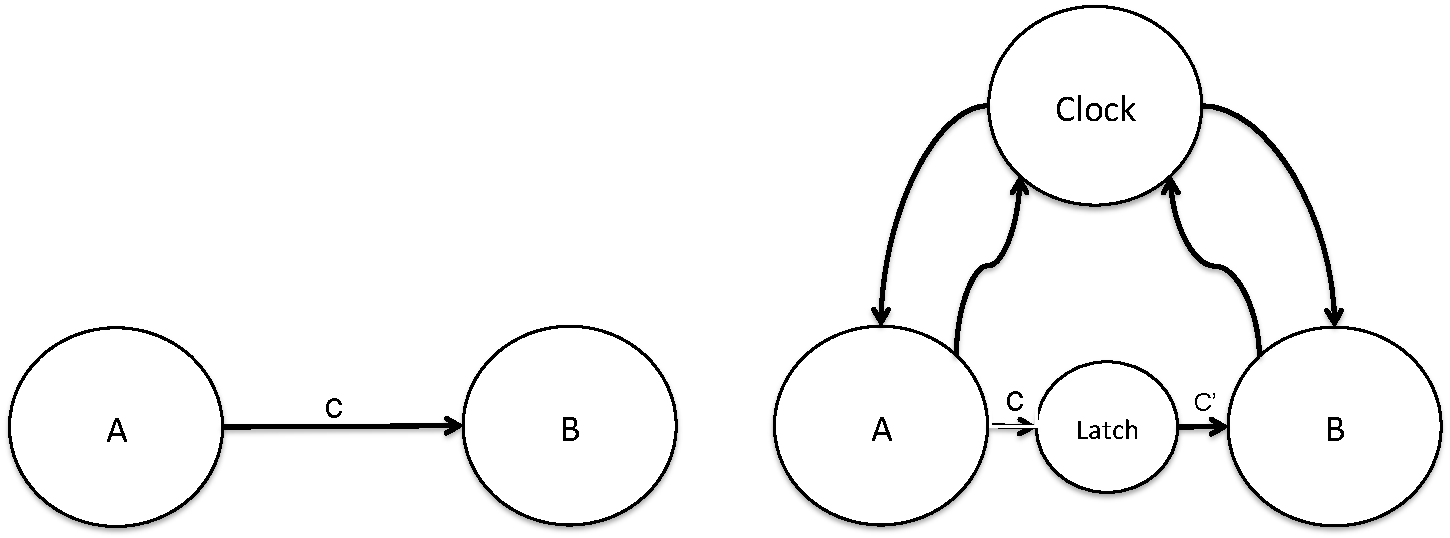
\includegraphics[width=0.9\textwidth]{figures/clocked.pdf}
  \caption{In order to enforce synchronous communication semantics on a simple
    CSP network, a large amount of additional complexity is needed. Figure
    from~\cite{vinter2014synchronous}.}
  \label{fig:clocked}
\end{figure}

The masters thesis project (mentioned above) which later attempted to convert
the CSP model to an actual hardware description found the pure CSP approach less
apt, revealing a fundamental discrepancy between the data propagation models of
hardware and of CSP. In CSP, a process is free to communicate whenever it wants
while in digital hardware, all communication is driven forward synchronously by
a clock.
% Enforcing globally synchronous communication using CSP is hard, since
% CSP is inherently asynchronous.
Thus, to accurately model hardware in CSP, this clock had to be emulated by
adding a single clock process with broadcasting channels to every other process
in the network. Back-channels also had to be inserted from every process in the
network to the clock process such that it could be informed when a process had
finished running. Furthermore, latch-processes had to be inserted into every
channel going between processes. This was needed in order to ensure that values
were not propagated in the middle of a clock cycle. The effect of adding these
additional processes and channels is seen in \Cref{fig:clocked}. Whenever the
clock process emitted a signal, all processes in the network would run. When the
processes had run, the latch processes ensured that values were propagated to
the next process.
% When all processes had signaled a completed
% run, the clock would signal the latch processes in order to propagate the values
% of the network.

In the end, the thesis successfully managed to translate simple PyCSP networks
to VivadoC, a language for HLS. Despite this, the conclusion of the thesis work
was that, while CSP could be forced to adhere by globally synchronous semantics,
the networks required to do so were prohibitively complex. Furthermore, only a
small subset of the features of CSP was used in the hardware-targeted
processes. Particularly, a concept central to CSP, \textit{external choice}
which allows a process to determine if it should run based on whether it
received a message, was not found to be applicable to hardware designs. However,
not all was bad: As concluded in the original vector-processor design work, the
shared-nothing property of CSP proved useful as the state of the network could
only be altered by processes communicating. This made it simple to compose
networks by making multiple instances of the same process.

These experiences discarded the idea of using pure CSP as a hardware design
tool, but lead to the conception of a derived model, SME, which maintained the
concepts of CSP that were found beneficial while adding a new, globally
synchronous, communication model. \cite{vinter2014synchronous}

\section{The Model}
The key concept of the SME model is that introducing an implicit clock would
eliminate the complexity of forcing CSP to adhere by globally synchronous
message. \todo{List properties}

\begin{description}
\item [Implicit clock]
\item[..]
\end{description}

\subsection{SME components}
Building on its CSP roots, the fundamental unit in an SME network is the
{\itshape process}. Processes are connected through buses, from which networks
are build. We use the name ``bus'' instead of ``channel'', which is used in CSP,
to maintain a hardware analogy and clarify its semantic equivalences with a
physical signal bus. Furthermore, a bus in SME generalize the concept of a wire

A bus in SME is equivalent to a collection of broadcasting channels.

A bus

% This is also considered part of the hardware analogy, since, is a bundle of
% wires which together constitute a combined signal path.

\subsection{Execution Flow}
The SME concept ``clock cycle'' (\Cref{fig:smeclock}) goes through two distinct
phases.
\begin{description}
\item[Compute phase.] All processes run during the compute phase. While the
  processes run, the values of the reading ends of buses are kept constant. 
\item[Bus propagation.] The bus propagation phase copies all values from the
  read-end of a bus to the write end.
\end{description}

Each channel in a bus has a reading-end and a writing-end. During the compute
phase of a cycle, the reading-ends of channels are kept constant. The writing
end of a channel has a single-element overwrite buffer. The bus propagation
phase copies all values from the reading-end to the writing end. Thus, values
written in cycle $c$, will be read in cycle $c+1$.

\begin{figure}
  \centering
\resizebox{.9\linewidth}{!}{
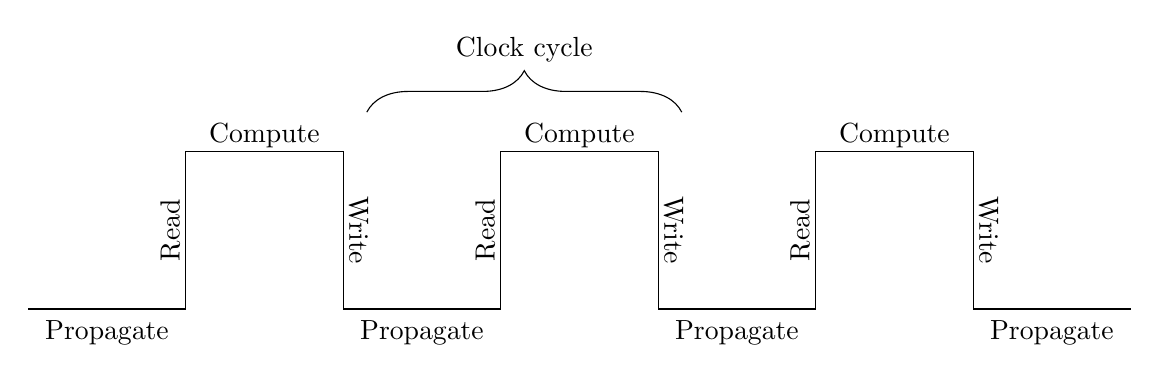
\begin{tikzpicture}
  \foreach \i in {0,4,8}
  \draw (\i,0) -- (\i+2,0) -- node [xshift=-0.2cm,rotate=90] {Read} (\i+2,2) -- node
  [yshift=0.2cm] {Compute}(\i+4,2) -- node [xshift=0.2cm,rotate=270] {Write} (\i+4,0);
  
  \draw (12,0) -- (14,0);
  \node [] at (13,-0.3) () {Propagate};

  \draw [decorate,decoration={brace,amplitude=15pt}] (4.3,2.5) -- (8.3,2.5) node
  [midway,yshift=0.8cm]{Clock cycle};

  \foreach \i in {0,4,8} {
  \node [] at (\i+1,-0.3) () {Propagate};
  % \node [blue] at (\i+3,-0.5) () {Run};
}

\end{tikzpicture}}
\caption{Illustration of the SME concept of the clock cycle}
\label{fig:smeclock}
\end{figure}


% Even though you may already have realized the properties and components of the
% SME model, we give a more formal introduction here.

% A clock signal has four different states. Its either low, raising, high or
% falling. Conceptually, SME processes reads their input on the raising edge, then
% does computation, before writing the result of the communication.

% As referenced previously, the CSP concept of external choice was not found to be
% a good fit for hardware design, The key insight of the SME model is the concept
% of a \textit{hidden clock}


\subsection{An intuition}
While describing the actions taken during an SME clock cycles is simple, gaining
an intuition of value propagation governed by globally synchronous semantics is
harder. We therefore show an example of a simple network, seen in
\Cref{fig:smeint}. We return to a slight variation of this example later, but
for now, the network consist of two processes $P_1$ and $P_2$ and two buses
connecting them, $b_1$ and $b_2$. In this network, a value is passed around in a
circular fashion. The $P_1$ and simply forwards the value it receives while the
$P_2$ process increments it by 1. In \Cref{tab:trace} we see the actual values
read and written by every process for every iteration. Note that before very
iteration, an implicit bus propagation is run, driving forward the bus
values. The arrows denote the operation performed. A process can either
{\itshape write into} or {\itshape read from} a bus. So, the operation
$P_1 \rightarrow b_1$ means that $P_1$ writes to $b_2$. The reading-ends of all
buses initially start out as 0. Thus, in the first cycle, both processes reads
the value . In the second cycle, we see the effect of the delayed data
propagation: $P_2$ reads 0 again, even though it wrote 1 in the last
iteration. The reason for this is that the 0 read now in cycle $c$ was written
by $P_1$ in cycle $c-1$.

\begin{figure}
  \centering
  \resizebox{.7\linewidth}{!}{
    \begin{tikzpicture}[font=\tiny,
      proc style/.style={circle,draw=black,align=center,text
        width=1cm,minimum size=1cm,align=center}
      ]
      \node[proc style] (id) {$=$};
      \node[below=0cm of id] (p1) {$P_1$};
      \node[proc style,right=2.5cm of id] (add) {$+1$};
      \node[below=0cm of add] (p2) {$P_2$};
      \draw[-{Latex[scale=1.6]}] (id) edge [bend left=30] node [above] {$b_2$} (add);
      \draw[-{Latex[scale=1.6]}] (add) edge [bend left=30] node [below] {$b_1$}
      (id);
    \end{tikzpicture}
    }
    \caption{A simple SME network consisting of two processes. One simply
      forwards the received value while the other increments it by one.}
  \label{fig:smeint}
\end{figure}

\begin{figure}
  \centering
  \begin{tabular}{c|cccccccccc}
    %\toprule
    \diagbox[height=1.6em]{op}{c} & 1 & 2 & 3 & 4 & 5 & 6 & 7 & 8 & 9  \\\hline
    $P_1 \leftarrow b_1$  & 0 & 1 & 1 & 2 & 2 & 3 & 3 & 4 & 4  \\
    $P_1 \rightarrow b_2$ & 0 & 1 & 1 & 2 & 2 & 3 & 3 & 4 & 4  \\
    $P_2 \leftarrow b_2$  & 0 & 0 & 1 & 1 & 2 & 2 & 3 & 3 & 4  \\
    $P_2 \rightarrow b_1$ & 1 & 1 & 2 & 2 & 3 & 3 & 4 & 4 & 5  \\
    %\bottomrule
  \end{tabular}
  \caption{A table showing values read and written for every clock cycle of SME
    networks. Note that when we refer to a {\itshape trace} later, it is
    different from the table shown here. An SME trace file normally only
    contains the values of the reading ends of bus channels following every
    cycle.}
\label{tab:trace}
\end{figure}

\begin{figure}
  \centering
  \resizebox{.7\linewidth}{!}{
    \begin{tikzpicture}[font=\tiny,
      proc style/.style={circle,draw=black,align=center,text
        width=1cm,minimum size=1cm,align=center}
      ]
      \node[proc style] (impl) {SME implementation};
      \node[proc style,right=0.7cm of impl] (sim) {Simulation};
      \node[proc style,right=1cm of sim] (tb) {Test bench};
      \node[proc style,above=0.5cm of tb] (trace) {CSV trace};
      \node[proc style,below=0.5cm of tb] (code) {VHDL Code};

      \node[gray,draw=gray,proc style,right=1cm of tb] (verifies) {Verifies};


      \draw[-{Latex[scale=1.6]}] (impl) edge [] (sim);
      \draw[-{Latex[scale=1.6]}] (sim) edge [] (trace);
      \draw[-{Latex[scale=1.6]}] (sim) edge [] (tb);
      \draw[-{Latex[scale=1.6]}] (sim) edge [] (code);

     \draw[-{Latex[scale=1.6]}] (trace) edge [gray, bend left=20] (verifies);
     \draw[-{Latex[scale=1.6]}] (tb) edge [gray] (verifies);
     \draw[-{Latex[scale=1.6]}] (verifies) edge [gray, bend left=20] (code);
 
    \end{tikzpicture}
    }
    \caption{A simplified overview of the steps taken by a SME implementation
      from  }
  \label{fig:smeflow}
\end{figure}

\section{Implementations}
A number of different SME implementations exists

The purpose of all ``model'' SME implementation is to eventually generate a
hardware description. The key advantage of SME is that a low-level hardware
description may be generated form an SME network written in a high-level
language. Furthermore, verification of the generated VHDL code is simplified
since also a test-bench is generated. An overview of the process is shown in
\Cref{fig:smeflow}. We show this, to give an understanding of what are the
phases of a normal SME workflow. First, an SME implementation written in a
general-purpose language is simulated, using a self-hosted simulator. A result
of this simulation is a trace file containing the values of the reading-ends of
buses for every cycle. The code is then translated to VHDL code and a test-bench
for testing the generated code. The test-bench will, using the values of the
trace file, cycle-for-cycle, test the generated code.

\subsection{\nth{1} PySME}

The initial implementation of SME was extremely simple: A mere 69 \gls{sloc} of
Python was all that was needed to create a library allowing Python programs to
be written following the SME model. This implementation was, of course, quite
rudimentary, however, it underlines a key advantage of the SME model. A person
can both understand the model and write a simulator from scratch in less than a
day.

Initially, SME was only used for simulation and prototyping of hardware
designs. The completed prototypes were then manually translated to
\gls{vhdl}. This was a tedious process, but it showed that performing such a
translation was viable and that implemeting. Automating this translation was
then the next focus


\subsection{\nth{2} PySME}
After an initial experience with the first version of PySME the SME model was
updated~\cite{vinter2015bus} to include some changes that was deemed useful. The
most noticeable change, was the abandonment of CSP-like single-value channels in
favor of Buses as described above. As buses were implemented as active
participants in the network (rather than just being an abstraction of process
read/write ports), it was now possible to use the buses to save a trace of the
values flowing through the network.

\subsection{C\# SME}
Based on the new version of SME, a C\# version of SME was also created. The
primary change compared to previous SME implementations is that the C\# version
lacks a ``Network''-like construct which is used purely for declaring the
relations between entities. Instead of being explicitly defined, connections
between a pair of processes was established if they reference the same bus. This
model made it easier to compose networks compared to PySME which required that
all buses and their use in connections had to be declared in a network
block. However, a shortcoming of this approach was that it made building
parameterized networks difficult. That is, one bus name in the code corresponded
one-to-one with a bus in the SME network. This problem was fixed in a later
version of C\# SME by the introduction of {\itshape scopes} which allowed
several instances of the same bus to exist as long as they were defined in
different scopes.

In the design of SMEIL, we have drawn
two conclusions from this. The first is, that requiring all buses and
connections to be declared in one place quickly become difficult to
understand. The other is, that it would be advantageous to create new bus
instances along with new process instances as they often have a fixed
relationship

\subsection{\nth{3} PySME}
Based on the success of translating SME models written in C\# to VHDL, a project
was started to bring the same capability to the Python version of SME. The
challenges of deriving static code from a dynamic language were briefly
mentioned in the introduction. Due to this, the previous PySME implementation
was altered to require more explicit code. For example \todo{show code} in the
\nth{2} PySME, declaring a bus could be done simply by creating a field in a
Network class. This made analyzing the code difficult, since the users intention
was not clearly stated. Thus, an {\ttfamily add} method was added to the
\texttt{Network} class.


%%% Local Variables:
%%% mode: latex
%%% TeX-master: "../master"
%%% End:
